% !TEX TS-program = pdflatex
% !TEX encoding = UTF-8 Unicode

\documentclass[12pt]{article} 

\usepackage[utf8]{inputenc} % set input encoding 
\usepackage{geometry} % to change the page dimensions
\geometry{a4paper} 
\usepackage[parfill]{parskip} % No indent in document

% Packages
\usepackage{graphicx}
\usepackage{array}
\usepackage{amsmath}
\usepackage{amssymb}
\usepackage{verbatim}
\usepackage{xcolor}
\usepackage[hidelinks]{hyperref}
\usepackage{tikz}

\usepackage{todonotes}
\setuptodonotes{inline, size=\small}

% Define colors
\definecolor{mint}{rgb}{0.65,0.84,0.82}
\definecolor{scheme}{rgb}{0,0,1}

\title{Bitcoin, Blockchain and Cryptoassets \\ Exercise Set 2}
\author{}
\date{ } 

\begin{document}
	\maketitle
	
	In this second exercise set, we will mainly cover the content of the lectures on transaction consensus. \par
	
	Keep in mind that solving this exercise set is voluntary and UNGRADED. The solutions are either shared already or will be in due time.
	
	\newpage
	
	\section*{Exercise 1}
	In this exercise you have to analyze several made up ideas for changes to the consensus protocol of the Bitcoin Blockchain. We ask you to determine the (protocol-based) fork type which this change implies and what happens when more miners apply the old or the new rule set.
	\subsection*{Exercise 1.1}
	The current maximal block size on the Bitcoin Blockchain is 1 MB (ignoring the segwit extension). Assume, that some miners want to increase the block size to 2 MB in order to double the number of transactions that can be processed per block. What kind of fork type would this change result in (ceteris paribus)? Will there likely occur a chain split if more computational resources are allocated to the new (a) or the old (b) consensus protocol? Why?
	
	\subsection*{Exercise 1.2}
	So far there is no minimal transaction fee in the Bitcoin Blockchain. Assume that, to ensure the remuneration of the miners, a Bitcoin Improvement Proposal (BIP) is released which implements a minimal transaction fee of 0.0015 BTC ($\approx$ CHF 75 at the time of writing this tutorial). What kind of fork type would this change result in (ceteris paribus)? Will there likely occur a chain split if more computational resources are allocated to the new (a) or the old (b) consensus protocol? Why?
	
	\subsection*{Exercise 1.3}
	Assume the next BIP plans to implement a new minimal block size of 0.5 MB\footnote{There can be incentives for miners not to include transactions in a block. One reason can be that smaller sized blocks are distributed faster in the network compared to a "normal" block of size 1 MB. Thus, a miner could try to outrun competing blocks at the cost of loosing the transaction fees.} and at the same time, a maximal block size of 2 MB. What kind of fork type would this change result in (ceteris paribus)? Will there likely occur a chain split if more computational resources are allocated to the new (a) or the old (b) consensus protocol? Why?
	
	\newpage
	\subsection*{Exercises 1.4}
	
	Categorize the following examples into their fork types to further deepen your understanding:
	
	\begin{itemize}
		\item[(a)] A change in the threshold value so that there are, on average, two blocks found per ten minutes.
		
		\item[(b)] A reduction of the remuneration of the miners via the coinbase transaction to maximal 5 BTC\footnote{Note that a miner could, in theory, award himself less than the maximal block reward.}
		
	%	\item[(c)] A change in the number of blocks to the next threshold adaption from 2,016 to 1,008 blocks. Thus the threshold would be adapted every seven days.
	%	
	\end{itemize}
	
	\section*{Exercise 2}
	
	Consider the network topology below. Eve initiates a transaction $X$ to node $D$ to pay for a coffee. At the same time, she initiates a second transaction $Y$ to node $B$ which references the same UTXO as transaction $X$ but is in favor of another of her own addresses. Her plan is, that transaction $Y$ will be included in the Blockchain, and that she will be long gone when the coffee place realizes, that her coffee-transaction was confirmed. This is one form of a double spend attack. The numbers in the nodes correspond to the respective computational resources used for mining. Assume, that the connections between the nodes are homogeneous\footnote{This means that it always takes the same time to send a message/transaction to reach the next node.}. Furthermore nodes will only consider the transaction that reaches them first in their block candidate and will forward only this transaction to connected nodes. Determine the probability that transaction $Y$ will be included in the next block and therefore the success of the double spend attack. Hint: Eve will use her mining power for transaction $Y$.
	
	\begin{figure}[h!]
		\centering
		\resizebox{11cm}{!}{
			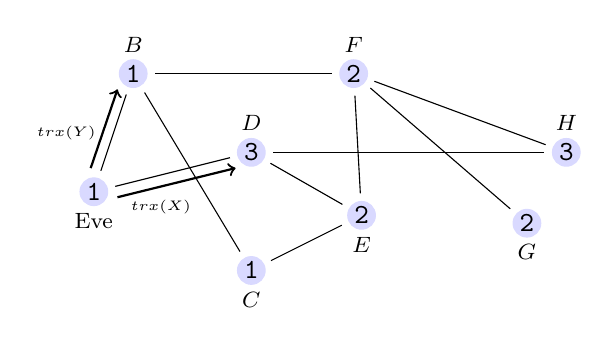
\begin{tikzpicture}[domain=-8:8]
				\coordinate (c1) at (5,0);%Edith
				\coordinate (c2) at (7,-1);%Tony
				\coordinate (c3) at (7,0.5);%Marcia
				\coordinate (c4) at (8.4,-0.3);%Mich\`eles
				\coordinate (c5) at (8.3,1.5);%Brian
				\coordinate (c6) at (11,0.5);%Jake
				\coordinate (c7) at (10.5,-0.4);%Claudia
				\coordinate (c8) at (5.5,1.5);%B
				\coordinate (z1) at (4.65,0.75);%trx(y)
				\coordinate (z2) at (5.85,-0.2);%trx(x)
				\filldraw[color=scheme!15] (c1) circle (5pt) node[color=black]{\texttt{1}} node[below=0.15cm,color=black]{\footnotesize{Eve}};
				\filldraw[color=scheme!15] (c2) circle (5pt) node[color=black]{\texttt{1}} node[below=0.15cm,color=black]{\footnotesize{$C$}};
				\filldraw[color=scheme!15] (c3) circle (5pt) node[color=black]{\texttt{3}} node[above=0.15cm,color=black]{\footnotesize{$D$}};
				\filldraw[color=scheme!15] (c4) circle (5pt) node[color=black]{\texttt{2}} node[below=0.15cm,color=black]{\footnotesize{$E$}};
				\filldraw[color=scheme!15] (c5) circle (5pt) node[color=black]{\texttt{2}} node[above=0.15cm,color=black]{\footnotesize{$F$}};
				\filldraw[color=scheme!15] (c6) circle (5pt) node[color=black]{\texttt{3}} node[above=0.15cm,color=black]{\footnotesize{$H$}};
				\filldraw[color=scheme!15] (c7) circle (5pt) node[color=black]{\texttt{2}} node[below=0.15cm,color=black]{\footnotesize{$G$}};
				\filldraw[color=scheme!15] (c8) circle (5pt) node[color=black]{\texttt{1}} node[above=0.15cm,color=black]{\footnotesize{$B$}};
				
				\draw[shorten >=0.28cm,shorten <=0.28cm] (c1) to[] (c3);
				\draw[shorten >=0.28cm,shorten <=0.28cm] (c1) to[] (c8);
				\draw[shorten >=0.28cm,shorten <=0.28cm] (c2) to[] (c4);
				\draw[shorten >=0.28cm,shorten <=0.28cm] (c2) to[] (c8);
				\draw[shorten >=0.28cm,shorten <=0.28cm] (c3) to[] (c4);
				\draw[shorten >=0.28cm,shorten <=0.28cm] (c3) to[] (c6);
				\draw[shorten >=0.28cm,shorten <=0.28cm] (c4) to[] (c5);
				\draw[shorten >=0.28cm,shorten <=0.28cm] (c5) to[] (c6);
				\draw[shorten >=0.28cm,shorten <=0.28cm] (c5) to[] (c7);
				\draw[shorten >=0.28cm,shorten <=0.28cm] (c5) to[] (c8);
				
				\draw [color = black,->,thick] (4.96,0.30) to (5.3,1.3);
				\node at (z1)[color=black]{\tiny{$trx(Y)$}};
				\draw [color = black,->,thick] (5.3,-0.07) to (6.8,0.3);
				\node at (z2)[color=black]{\tiny{$trx(X)$}};
				
		\end{tikzpicture}}
	\end{figure}
	\newpage
	
	\section*{Exercise 3}
	
	Consider the same network topology as before:
	
	\begin{figure}[h!]
		\centering
		\resizebox{10cm}{!}{
			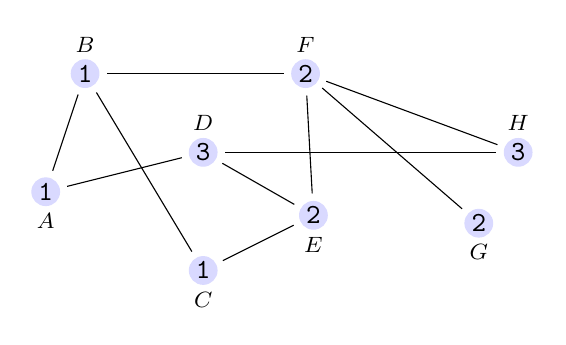
\begin{tikzpicture}[domain=-8:8]
				\coordinate (c1) at (5,0);%Edith
				\coordinate (c2) at (7,-1);%Tony
				\coordinate (c3) at (7,0.5);%Marcia
				\coordinate (c4) at (8.4,-0.3);%Mich\`eles
				\coordinate (c5) at (8.3,1.5);%Brian
				\coordinate (c6) at (11,0.5);%Jake
				\coordinate (c7) at (10.5,-0.4);%Claudia
				\coordinate (c8) at (5.5,1.5);%Tamara
				\filldraw[color=scheme!15] (c1) circle (5pt) node[color=black]{\texttt{1}} node[below=0.15cm,color=black]{\footnotesize{$A$}};
				\filldraw[color=scheme!15] (c2) circle (5pt) node[color=black]{\texttt{1}} node[below=0.15cm,color=black]{\footnotesize{$C$}};
				\filldraw[color=scheme!15] (c3) circle (5pt) node[color=black]{\texttt{3}} node[above=0.15cm,color=black]{\footnotesize{$D$}};
				\filldraw[color=scheme!15] (c4) circle (5pt) node[color=black]{\texttt{2}} node[below=0.15cm,color=black]{\footnotesize{$E$}};
				\filldraw[color=scheme!15] (c5) circle (5pt) node[color=black]{\texttt{2}} node[above=0.15cm,color=black]{\footnotesize{$F$}};
				\filldraw[color=scheme!15] (c6) circle (5pt) node[color=black]{\texttt{3}} node[above=0.15cm,color=black]{\footnotesize{$H$}};
				\filldraw[color=scheme!15] (c7) circle (5pt) node[color=black]{\texttt{2}} node[below=0.15cm,color=black]{\footnotesize{$G$}};
				\filldraw[color=scheme!15] (c8) circle (5pt) node[color=black]{\texttt{1}} node[above=0.15cm,color=black]{\footnotesize{$B$}};
				
				\draw[shorten >=0.28cm,shorten <=0.28cm] (c1) to[] (c3);
				\draw[shorten >=0.28cm,shorten <=0.28cm] (c1) to[] (c8);
				\draw[shorten >=0.28cm,shorten <=0.28cm] (c2) to[] (c4);
				\draw[shorten >=0.28cm,shorten <=0.28cm] (c2) to[] (c8);
				\draw[shorten >=0.28cm,shorten <=0.28cm] (c3) to[] (c4);
				\draw[shorten >=0.28cm,shorten <=0.28cm] (c3) to[] (c6);
				\draw[shorten >=0.28cm,shorten <=0.28cm] (c4) to[] (c5);
				\draw[shorten >=0.28cm,shorten <=0.28cm] (c5) to[] (c6);
				\draw[shorten >=0.28cm,shorten <=0.28cm] (c5) to[] (c7);
				\draw[shorten >=0.28cm,shorten <=0.28cm] (c5) to[] (c8);
		\end{tikzpicture}}
	\end{figure}
	\subsection*{Exercise 3.1}
	\begin{itemize}
		\item[a)] Compute the expected payoff $\mathbb{E}[R]$ for miner $H$ from the next block that is found (in general). The current block reward is 6.25 BTC. Ignore transaction fees possibly included in the block.
		\item[b)] Compute the corresponding standard deviation of the payoff to miner $H$.
	\end{itemize}
	
	\subsection*{Exercise 3.2}
	
	In the next step we assume that the miners $E$, $F$ and $G$ revoke their connections to all nodes and instead join a mining pool hosted by miner $H$. For simplicity we assume that there are no fees for joining the mining pool.
	
	\begin{itemize}
		\item[a)] Compute again the expected payoff of miner $H$ from the next block that is found. Assume, that the payoff within the mining pool is divided proportional to the computational resources they contribute to the pool (i.e. if the pool finds a block, miner $F$ receives $\frac{2}{9} \cdot 6.25$)
		\item[b)] Compute the corresponding standard deviation of the expected payoff to miner $H$.
		\item[c)] As a last step, can you think of reasons why the consolidation of these four miners into a pool could be problematic for our small example network?
	\end{itemize}
	
	\newpage
	
	\section*{Exercise 4}
	
	\subsection*{Exercise 4.1}
	
	Consider the scenario depicted in the figure below\footnote{The content of exercise 4 was not covered in the lecture. However it can be found in the (exam relevant) book of the lecture on pages 163 (engl.) or 228 (de).}. Michèle and Tony have found a block at the same time, but since then, two blocks were added based on Michèle's block. Tony is very unhappy about this, as he has lost the block reward included in his block because of this. Therefore, he could try to save his initial block reward by finding three consecutive blocks and overtaking the chain with Michèle's block. Compute the relative hash rate $\frac{h}{H}$ of Tony with which he would be indifferent between trying to safe his initial block reward and continuing at the current state of Michèle's chain. Hint: set the expected payoff of Tony's two options equal and solve for the relative hash rate.
	
	\begin{figure}[h!]
		\centering
		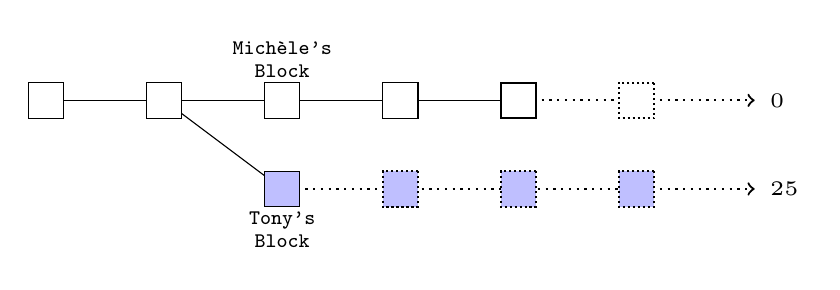
\begin{tikzpicture}[domain=1:10,scale=1.5, every node/.style={scale=1.5}]
			\coordinate (o1) at (1,1);
			\coordinate (o2) at (2,1);
			\coordinate (o3) at (3,1);
			\coordinate (o4) at (4,1);
			\coordinate (o5) at (5,1);
			\coordinate (o6) at (6,1);
			\coordinate (o7) at (7,1);
			\coordinate (o8) at (8,1);
			\coordinate (o9) at (9,1);
			\coordinate (o10) at (10,1);
			\coordinate (n1) at (1,0.25);
			\coordinate (n2) at (2,0.250);
			\coordinate (n3) at (3,0.250);
			\coordinate (n4) at (4,0.250);
			\coordinate (n5) at (5,0.250);
			\coordinate (n6) at (6,0.250);
			\coordinate (n7) at (7,0.250);
			\coordinate (n8) at (8,0.250);
			\coordinate (n9) at (9,0.250);
			\coordinate (n10) at (10,0.250);
			
			\draw[] (o1) -- (o2) -- (o3) -- (o4) -- (o5);
			\draw[] (o2) -- (n3); 
			\draw[dotted, thick] (n3) -- (n4) -- (n5) -- (n6);
			\draw[dotted, thick] (o5) -- (o6);
			\draw[color=black,thick, dotted, ->] (o6) to[] (o7) node[right]{\tiny{$0$}};
			\draw[color=black,thick, dotted, ->] (n6) to[] (n7) node[right]{\tiny{$25$}};
			
			\node (rect) at (o1) [fill=white,draw,minimum width=0.3cm,minimum height=0.3cm] {};
			\node (rect) at (o2) [fill=white,draw,minimum width=0.3cm,minimum height=0.3cm] {};
			\node (rect) at (o3) [fill=white,draw,minimum width=0.3cm,minimum height=0.3cm] {};
			\node (rect) at (o4) [fill=white,draw,minimum width=0.3cm,minimum height=0.3cm] {};
			\node at (o3) [above=0.1cm]{\tiny{\texttt{Block}}};
			\node at (o3) [above=0.4cm]{\tiny{\texttt{Mich\`ele's}}};
			\node at (n3) [below=0.4cm]{\tiny{\texttt{Block}}};
			\node at (n3) [below=0.1cm]{\tiny{\texttt{Tony's}}};
			\node (rect) at (o5) [fill=white,thick,draw,minimum width=0.3cm,minimum height=0.3cm] {};
			\node (rect) at (o6) [thick, densely dotted, fill=white,draw,minimum width=0.3cm,minimum height=0.3cm] {};
			\node (rect) at (n3) [fill=scheme!25,draw,minimum width=0.3cm,minimum height=0.3cm] {};
			\node (rect) at (n4) [thick,fill=scheme!25,draw,minimum width=0.3cm,minimum height=0.3cm,densely dotted] {};
			\node (rect) at (n5) [thick,fill=scheme!25,draw,minimum width=0.3cm,minimum height=0.3cm,densely dotted] {};
			\node (rect) at (n6) [thick, densely dotted, fill=scheme!25,draw,minimum width=0.3cm,minimum height=0.3cm] {};
		\end{tikzpicture}
	\end{figure}
	\vspace{-1cm}
	\subsection*{Exercise 4.2}
	
	In this exercise we slightly alter the story above. Now, we assume that there is only one additional block in Michèle's chain. In addition to that we assume that there were unusually high transaction fees included in the two initially found blocks by Tony and Michèle. We denote these high transaction fees with $f > 0$. All remaining blocks will only include the usual transaction fees, which we assume to be zero for simplicity and thus only consider the block reward $R$ for these blocks. Formulate again the indifference equation for Tony and solve for the transaction fee $f$. Which relation between $f$ and $R$ results if we assume that Tony controls 20\% of the network hash rate ($\frac{h}{H} = \frac{1}{5}$)?
	
	\begin{figure}[h!]
		\centering
		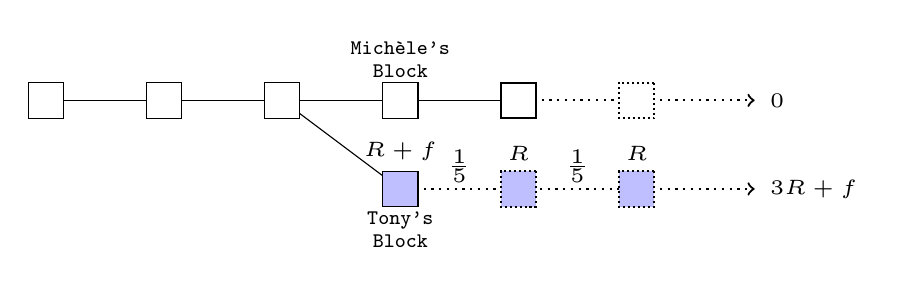
\begin{tikzpicture}[domain=1:10,scale=1.5, every node/.style={scale=1.5}]
			\coordinate (o1) at (1,1);
			\coordinate (o2) at (2,1);
			\coordinate (o3) at (3,1);
			\coordinate (o4) at (4,1);
			\coordinate (o5) at (5,1);
			\coordinate (o6) at (6,1);
			\coordinate (o7) at (7,1);
			\coordinate (o8) at (8,1);
			\coordinate (o9) at (9,1);
			\coordinate (o10) at (10,1);
			\coordinate (n1) at (1,0.25);
			\coordinate (n2) at (2,0.250);
			\coordinate (n3) at (3,0.250);
			\coordinate (n4) at (4,0.250);
			\coordinate (n5) at (5,0.250);
			\coordinate (n6) at (6,0.250);
			\coordinate (n7) at (7,0.250);
			\coordinate (n8) at (8,0.250);
			\coordinate (n9) at (9,0.250);
			\coordinate (n10) at (10,0.250);
			
			\draw[] (o1) -- (o2) -- (o3) -- (o4) -- (o5) ;
			\draw[] (o3) -- (n4); 
			\draw[dotted, thick] (n4) -- (n5) node[midway, yshift=0.19cm]{\tiny{$\frac{1}{5}$}} -- (n6) node[midway, yshift=0.19cm]{\tiny{$\frac{1}{5}$}} ;
			\draw[dotted, thick] (o5) -- (o6);
			\draw[color=black,thick, dotted, ->] (o6) to[] (o7) node[right]{\tiny{$0$}};
			\draw[color=black,thick, dotted, ->] (n6) to[] (n7) node[right]{\tiny{\(3R+f\)}};
			
			\node (rect) at (o1) [fill=white,draw,minimum width=0.3cm,minimum height=0.3cm] {};
			\node (rect) at (o2) [fill=white,draw,minimum width=0.3cm,minimum height=0.3cm] {};
			\node (rect) at (o3) [fill=white,draw,minimum width=0.3cm,minimum height=0.3cm] {};
			\node (rect) at (o4) [fill=white,draw,minimum width=0.3cm,minimum height=0.3cm] {};
			\node at (o4) [above=0.1cm]{\tiny{\texttt{Block}}};
			\node at (o4) [above=0.4cm]{\tiny{\texttt{Mich\`ele's}}};
			\node at (n4) [below=0.4cm]{\tiny{\texttt{Block}}};
			\node at (n4) [below=0.1cm]{\tiny{\texttt{Tony's}}};
			
			\node at (n4) [above=0.175cm,color=black]{\tiny{\(R+f\)}};
			\node at (n5) [above=0.175cm,color=black]{\tiny{\(R\)}};
			\node at (n6) [above=0.175cm,color=black]{\tiny{\(R\)}};
			
			\node (rect) at (o5) [fill=white,thick,draw,minimum width=0.3cm,minimum height=0.3cm] {};
			\node (rect) at (o6) [thick, densely dotted, fill=white,draw,minimum width=0.3cm,minimum height=0.3cm] {};
			\node (rect) at (n4) [fill=scheme!25,draw,minimum width=0.3cm,minimum height=0.3cm] {};
			\node (rect) at (n5) [thick,fill=scheme!25,draw,minimum width=0.3cm,minimum height=0.3cm,densely dotted] {};
			\node (rect) at (n6) [thick, densely dotted, fill=scheme!25,draw,minimum width=0.3cm,minimum height=0.3cm] {};
		\end{tikzpicture} 
	\end{figure}
	
\end{document}